\documentclass[11pt]{article}
\usepackage[preprint]{acl}
\usepackage{times}
\usepackage{latexsym}
\usepackage[T1]{fontenc}
\usepackage[utf8]{inputenc}
\usepackage{microtype}
\usepackage{inconsolata}
\usepackage{graphicx}
\usepackage{booktabs}
\usepackage{amsmath}

\newcommand{\om}[1]{\textit{#1}}

\title{Building an Afaan Oromoo Language Model from Scratch:\\Data, Tokenization, Pretraining and Adaptation on a Laptop}

\author{Habtamu Feyera \\
  Independent researcher \\
  % TODO: add email and affiliation if desired
}

\begin{document}
\maketitle

\begin{abstract}
We build a complete language-model pipeline for Afaan Oromoo, a widely spoken but under-resourced Cushitic language, on a single laptop (Apple M1 Max). Following the from-scratch recipe of \citet{raschka2025build}, we adapt each stage to Oromo: a 12.76M-word cleaned corpus that adds 19 public Telegram news channels to AfriBERTa and Wikipedia, filtered so that no evaluation headline or article text appears in training; a byte-level BPE tokenizer that keeps the hudhaa (\texttt{'}) inside words and halves sequence length relative to GPT-2 (4.98 vs.\ 2.34 characters per token); and a 23M-parameter GPT pretrained in 77 minutes to 1.50 bits per character. Growing the corpus from 6.9M to 12.8M words improves held-out text from every source.
Fine-tuned for news-topic classification on MasakhaNEWS, the pretrained model reaches 87.8\% accuracy and 0.809 macro-F1, against 0.577 for the same architecture trained from random weights and 0.749 for TF-IDF with logistic regression. Instruction tuning on 3,758 examples built from real Oromo text teaches the 23M model the answer format but not reliably to use its input; the same data with LoRA on an Oromo-adapted 0.8B model reaches 91.1\% topic accuracy and beats a lead baseline on headlines.
Comparing open models in bits per character, our 23M model outperforms a general 752M multilingual model by almost $2\times$ (1.49 vs.\ 2.88 on validation text), while the same 752M model after African-language continued pretraining is best on every test set, most clearly on 658 posts published after its release (1.15 vs.\ 1.54 for ours). LoRA continued pretraining of Qwen3-0.6B on 2.5M Oromo tokens cuts its bits per character by 40--49\%. The results point to Oromo-specific data and tokenization, more than model size, as the main levers for small-scale Oromo language modeling, and to model size as the limit for instruction following. Code: \url{https://github.com/HabtamuFeyera/afaan-oromoo-llm}.
\end{abstract}

\section{Introduction}

Afaan Oromoo is one of the most widely spoken languages in Africa, yet it has little digital text and few language models. General-purpose tokenizers and models are built mostly from English and other high-resource languages. They split Oromo words into many fragments and often fail to produce Oromo at all: prompted with \om{Afaan Oromoo}, a general 752M-parameter model continued in Afrikaans in our tests.

This paper asks how far a single researcher with a laptop can get by building every stage for Oromo from the ground up. We follow the open, from-scratch GPT recipe of \citet{raschka2025build} and change what Oromo needs changed: the data, the tokenizer, the model size, the evaluation and the instruction data. We then compare the result with open multilingual models. We address four questions:
\begin{enumerate}
\item \textbf{Tokenization:} how much does an Oromo-specific tokenizer save over GPT-2's English-centric one?
\item \textbf{Pretraining at small scale:} what can a 23M-parameter model learn from about 21M tokens of Oromo, and how much does more data help?
\item \textbf{Transfer:} does that pretraining help downstream tasks, and does instruction tuning work at this scale?
\item \textbf{Data versus size:} how does a small Oromo-only model compare with larger open models, before and after Oromo adaptation?
\end{enumerate}

\noindent Our contributions are:
\begin{itemize}
\item A reproducible cleaning pipeline for Oromo text that unifies the hudhaa, removes news-site boilerplate, imports Telegram channel exports, and removes evaluation text from training at both the 13-gram and the headline level.
\item A byte-level BPE tokenizer that keeps the hudhaa inside words, with a vocabulary-size study.
\item A 23M-parameter Oromo GPT evaluated on language modeling, topic classification and instruction following, with baselines, multiple seeds and a corpus-size ablation.
\item A tokenizer-independent comparison (bits per character) with general and Africa-adapted open models, including our own LoRA continued pretraining.
\item An instruction dataset built from real Oromo text rather than translation, and an analysis of what instruction tuning does and does not achieve at 23M parameters.
\end{itemize}

\section{Related Work}

\paragraph{Language models for African languages.} AfriBERTa \citep{ogueji2021afriberta} showed that small encoder models pretrained only on African languages can match much larger multilingual models; its corpus is our main public pretraining source. MasakhaNEWS \citep{adelani2023masakhanews} provides news-topic classification for 16 African languages, including Oromo, which we use for downstream evaluation. AfriqueLLM \citep{yu2026afriquellm} continues pretraining open decoder models on African languages, Oromo included; we use its 0.8B model as a reference point.

\paragraph{Tokenization.} Byte pair encoding \citep{sennrich2016bpe} and its byte-level form in GPT-2 \citep{radford2019gpt2} learn subwords from frequency, so languages rare in the training data are split into short fragments. An existing 12k byte-level BPE tokenizer for Oromo trained on AfriBERTa \citep{naolbm_oromo_bbpe} is our tokenizer baseline.

\paragraph{Small models and limited data.} Our pretraining recipe follows \citet{raschka2025build}. \citet{muennighoff2023scaling} show that repeating data for up to about four epochs costs little compared with fresh data, which motivates our four passes over a fixed corpus.

\paragraph{Contamination.} We follow the 13-gram overlap test of \citet{brown2020gpt3} to check evaluation sets against pretraining data, and add whole-phrase matching for headlines, which are usually shorter than 13 words.

\paragraph{Instruction tuning and adaptation.} We build instruction data from existing labeled and structured text, as FLAN did \citep{wei2022flan,longpre2023flan}, and use an Alpaca-style prompt \citep{taori2023alpaca}. For adapting larger models we use LoRA \citep{hu2022lora}.

\section{Data}
\label{sec:data}

The pretraining corpus has 12.76M words of cleaned Oromo text from three sources (Table~\ref{tab:data}), plus held-out validation sets that no training text overlaps.

\begin{table}[t]
\centering
\small
\begin{tabular}{@{}lrr@{}}
\toprule
Source & Docs & Words \\
\midrule
AfriBERTa, Oromo subset & sentences & 6.52M \\
Oromo Wikipedia (Nov 2023) & 1,772 & 0.36M \\
Telegram, 19 channels (2019--2026) & 136,420 & 5.87M \\
\midrule
Total & & 12.76M \\
\bottomrule
\end{tabular}
\caption{Training text by source. AfriBERTa is Apache-2.0 and Wikipedia CC BY-SA 4.0. Telegram posts (the largest channels are FMC, OBN, Burqaa Ispoortii, TIKVAH, BBC Afaan Oromoo, Jawar Mohammed and Addis Standard) remain under their channels' copyright and are used locally only.}
\label{tab:data}
\end{table}

\paragraph{Cleaning.} Every line is normalized and filtered by the same rules. \emph{Hudhaa:} the raw AfriBERTa text writes the glottal-stop apostrophe two ways almost equally often (189k ASCII \texttt{'} and 173k U+2019), so a model would see two spellings of words like \om{baay'ee}; all apostrophe variants are mapped to ASCII \texttt{'}. \emph{Boilerplate:} links, Wikipedia citation marks, BBC photo-caption labels (\om{Madda suuraa}, \om{Ibsa waa'ee suuraa}) and site menus are removed, keeping the surrounding sentence. \emph{Filters:} lines are dropped if they have fewer than 3 words, contain Cyrillic or Arabic script, are more than 10\% Ethiopic, are mostly non-letters, or are mostly English function words. \emph{Deduplication:} exact duplicates are removed, ignoring case and punctuation; validation text is processed first, so a repeated line is always removed from training. A sample of every dropped rule is written out for review; a first pass dropped real sentences that began with a caption label, ended in an ellipsis or quoted a short English phrase, and fixing these rules recovered about 2\% of the text.

\paragraph{Telegram channels.} Public channel histories were exported with Telegram Desktop: 19 channels of news, sports, government communication and commentary, with 215k posts that contain text. Before import, each channel was profiled for language, recurring lines, topics and overlap with the rest of the corpus. Hashtags, handles, emojis and links are removed, and styled Unicode letters (often used in sports posts) are folded to plain letters with NFKC. Any line that appears in three or more posts of a channel is treated as a signature and removed (391k lines, mostly social-media link blocks, sign-offs and reporter bylines). When a channel was exported twice, only the larger export is used. Telegram text is appended last, so the validation set is identical to that of the public-text corpus.

\paragraph{Contamination.} Any Telegram post that shares a single 13-word sequence with the validation set or the MasakhaNEWS dev and test articles is dropped (305 posts, mostly from BBC Afaan Oromoo, whose articles MasakhaNEWS is built from). Headlines are usually shorter than 13 words, so we also match MasakhaNEWS dev and test headlines as whole phrases, ignoring case and punctuation, and remove every training line or post that contains one (488 AfriBERTa lines and 33 posts). Before this filter, 81 of the 325 test headlines appeared verbatim in the public-text corpus, all through AfriBERTa. In the final corpus no test headline appears, and only 1 of 325 test articles has at least half of its 13-grams in the training text; on average 5.3\% do.

\paragraph{Splits.} Validation consists of the AfriBERTa evaluation split and 5\% of Wikipedia articles (0.51M words). A separate Telegram validation set holds 5\% of posts, chosen by a hash of channel and post id (7,334 posts, 0.32M words).

\section{Tokenization}
\label{sec:tok}

An Oromo byte-level BPE tokenizer with a 16k vocabulary halves sequence length relative to GPT-2 (Table~\ref{tab:tok}).

\paragraph{Design.} We train byte-level BPE, as in GPT-2, so no input is out of vocabulary. GPT-2's pre-tokenizer always splits at an apostrophe, which in Oromo cuts words such as \om{deebi'uun} and \om{ta'a} in two. Our pre-tokenizer keeps the hudhaa inside a word (\verb| ?\p{L}+(?:'\p{L}+)*|, followed by GPT-2's number, punctuation and whitespace patterns) and still separates quote marks at word edges. The sentence \om{Afaan Oromoo afaan ummata Oromoo kan Gaanfa Afrikaa keessa jiraatuuti.} takes 28 tokens with GPT-2 and 12 with ours. The tokenizer is trained on the public-text part of the corpus (AfriBERTa and Wikipedia).

\begin{table}[t]
\centering
\small
\setlength{\tabcolsep}{4pt}
\begin{tabular}{@{}lrrrrr@{}}
\toprule
Tokenizer & Vocab & C/T$\uparrow$ & T/W$\downarrow$ & 1-tok$\uparrow$ & Rare$\downarrow$ \\
\midrule
GPT-2 & 50,257 & 2.34 & 3.29 & 7.5 & 91.2 \\
Oromo-BBPE & 12,000 & 4.59 & 1.68 & 66.7 & 7.9 \\
Ours 8k & 8,000 & 4.47 & 1.73 & 64.4 & 1.5 \\
\textbf{Ours 16k} & 16,000 & \textbf{4.98} & \textbf{1.55} & \textbf{73.8} & 2.8 \\
Ours 24k & 24,000 & 5.24 & 1.47 & 78.5 & 4.5 \\
Ours 32k & 32,000 & 5.41 & 1.42 & 81.5 & 29.5 \\
\bottomrule
\end{tabular}
\caption{Tokenizers on the validation text. C/T: characters per token; T/W: tokens per word; 1-tok: \% of word occurrences that are a single token; Rare: \% of the vocabulary seen fewer than 50 times in training.}
\label{tab:tok}
\end{table}

\paragraph{Vocabulary size.} We choose 16k. Moving to 24k shortens sequences by only 5\% but adds 50\% more embedding parameters. At 32k, 29.5\% of the vocabulary is seen fewer than 50 times, too rarely for a small model to learn. Our 16k tokenizer also compresses Oromo 8\% better than the existing 12k Oromo tokenizer. With it, the training corpus is 21.45M tokens, against 44.6M with GPT-2.

\section{Pretraining}
\label{sec:pretrain}

\paragraph{Model.} We use the GPT architecture of \citet[ch.~4]{raschka2025build} unchanged: pre-LayerNorm transformer blocks with GELU feed-forward layers, learned absolute position embeddings and no weight tying, with 6 layers, 6 heads, width 384, a 256-token context (about 1,270 characters) and 23.0M parameters. Attention uses PyTorch's fused scaled-dot-product kernel, which we test to be numerically identical to the book's mask-and-softmax code. We train with AdamW (weight decay 0.1, peak learning rate $6\times10^{-4}$, 2\% linear warmup, cosine decay to 10\%, gradient clipping at 1.0) on batches of $32\times256$ tokens for four passes over the corpus, at about 20k tokens/s on an Apple M1 Max GPU.

\paragraph{Runs.} Our model trains on the full corpus: 21.45M tokens, 10,472 steps, 77 minutes. To measure the value of the data, we train the same model with the same settings, also for four passes, on two smaller versions of the corpus: the public text only (6.90M words) and the public text plus the first four Telegram channels we collected (8.05M words). All runs keep the checkpoint with the lowest validation loss. Validation loss improves at every checkpoint of every run and is still falling when training stops (Figure~\ref{fig:loss}).

\begin{figure}[t]
\centering
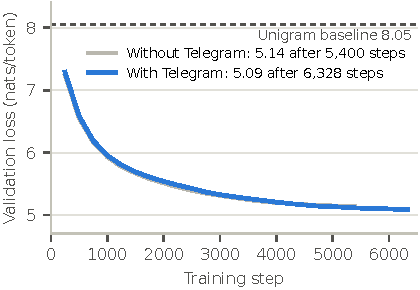
\includegraphics[width=\columnwidth]{figures/val_loss.pdf}
\caption{Validation loss of the same model on three corpus sizes, four passes each. Larger corpora get longer learning-rate schedules, so at equal steps they trail slightly, but they end lowest. Loss on 40 validation batches every 250 steps.}
\label{fig:loss}
\end{figure}

\begin{table}[t]
\centering
\small
\setlength{\tabcolsep}{3pt}
\begin{tabular}{@{}lrrrrrr@{}}
\toprule
& \multicolumn{2}{c}{Validation} & \multicolumn{2}{c}{Telegram-4} & \multicolumn{2}{c}{Telegram-19} \\
\cmidrule(lr){2-3}\cmidrule(lr){4-5}\cmidrule(l){6-7}
Training text & PPL & BPC & PPL & BPC & PPL & BPC \\
\midrule
Unigram & 3,421 & 2.43 & -- & -- & -- & -- \\
Public, 6.9M & 171 & 1.536 & 217 & 1.516 & 217 & 1.550 \\
+4 ch., 8.1M & 163 & 1.522 & 96 & 1.286 & 117 & 1.372 \\
+19 ch., 12.8M & \textbf{150} & \textbf{1.496} & \textbf{64} & \textbf{1.173} & \textbf{38} & \textbf{1.047} \\
\bottomrule
\end{tabular}
\caption{Language modeling on held-out text by training-corpus size (words). Telegram-4 and Telegram-19: held-out posts of the first four channels and of all 19. Perplexity is per token of our tokenizer; bits per character (BPC) is tokenizer-independent. The last row is our model.}
\label{tab:lm}
\end{table}

\paragraph{Results.} Table~\ref{tab:lm} reports perplexity and bits per character. More data helps on every held-out set, including the public validation text, which the added Telegram news does not resemble: its bits per character fall from 1.536 to 1.496. On held-out Telegram posts the gain is much larger (1.516 to 1.173 on the first four channels), because the added text covers 2019--2026 events, administration and sports that the public text lacks. Two caveats apply. Larger corpora also mean more optimizer steps at four passes each, so data and compute grow together. And Telegram validation posts come from the same channels as the training posts; channels repost similar stories in different words, which makes these sets easier than truly new text.

\paragraph{Samples.} Generations at temperature 0.7 are fluent-looking news Oromo with correct hudhaa forms and quoting style, but their content is invented: \om{Fayyaa hawaasaa guddisuuf mootummaan deeggarsa taasise. Deeggarsichi \dots\ manneen harka qalleeyyiif deeggarsa nyaataa kennuuf dandeessisuu ibseera.} (``The government provided support to improve public health. The support \dots\ enables food aid to low-income households.''), followed by an invented amount of money. At temperature 0 the model loops (\om{Afaan Oromoo, Afaan Oromoo, \dots}). Every word generated in our samples at temperature 0.7 occurs in the training text.

\section{Topic Classification}
\label{sec:cls}

\paragraph{Task.} MasakhaNEWS Oromo assigns BBC Afaan Oromoo articles to five topics, with 1,128 training, 162 dev and 325 test articles. Topics are unbalanced (technology has only 50 training articles), so we report macro-F1 alongside accuracy. The model reads the headline and the start of the article, cut to the 256-token context.

\paragraph{Method.} Following \citet[ch.~6]{raschka2025build}, the 16k-word output layer is replaced by a 5-class head, and the class is read at the last real token. We compare a majority-class baseline; TF-IDF word uni- and bigrams with logistic regression (C tuned on dev); and the GPT trained from random initialization, from pretraining with only the last block, final norm and head trained (the book's recipe, 1.8M parameters), and from pretraining with all layers trained (16.9M parameters). Each GPT setup tries learning rates $\{5\times10^{-5}, 2\times10^{-4}, 5\times10^{-4}\}$ for up to 10 epochs, keeps the best epoch on dev macro-F1, and reruns the best rate with 3 seeds.

\begin{figure}[t]
\centering
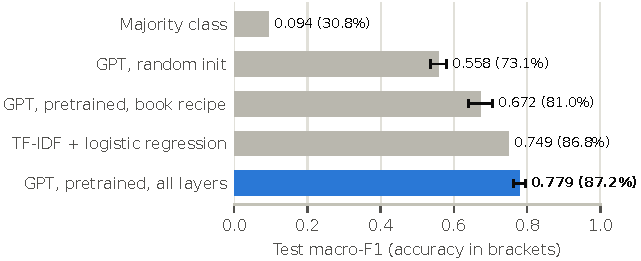
\includegraphics[width=\columnwidth]{figures/topic_f1.pdf}
\caption{Pretraining raises test macro-F1 from 0.58 to 0.81, above TF-IDF (0.75). GPT systems: mean of 3 seeds, whiskers $\pm1$ SD.}
\label{fig:f1}
\end{figure}

\begin{table}[t]
\centering
\small
\begin{tabular}{@{}lrrr@{}}
\toprule
Topic (train) & TF-IDF & GPT rand. & GPT pretr. \\
\midrule
Sports (280) & \textbf{0.98} & 0.88 & 0.96 \\
Health (338) & 0.88 & 0.81 & \textbf{0.89} \\
Politics (350) & 0.87 & 0.75 & \textbf{0.89} \\
Entertainment (110) & 0.60 & 0.29 & \textbf{0.63} \\
Technology (50) & 0.42 & 0.15 & \textbf{0.67} \\
\bottomrule
\end{tabular}
\caption{F1 per topic (GPT systems: all layers trained, mean of 3 seeds).}
\label{tab:pertopic}
\end{table}

\paragraph{Results.} Pretraining is what makes the model competitive (Figure~\ref{fig:f1}): macro-F1 rises from 0.577 to 0.809 and accuracy from 74.1\% to 87.8\%, above TF-IDF in macro-F1 (0.749) and level with it in accuracy (86.8\%). The gain is largest on rare topics (Table~\ref{tab:pertopic}): technology F1 rises from 0.15 to 0.67, well above TF-IDF's 0.42, because the model has already seen their vocabulary in unlabeled text. TF-IDF still wins on sports, where team and player names decide the topic. Training a tenth of the parameters (the book's recipe) reaches 86.1\% and 0.753, three quarters of the gain over random initialization. Corpus size matters most in that setting: with the public-text model as the starting point, the book's recipe reaches only 81.0\% and 0.672, while training all layers reaches 87.2\% and 0.779. Removing the one test article found in the training text changes no score at three decimals.

\section{Instruction Tuning}
\label{sec:inst}

\paragraph{Data.} No Oromo instruction dataset exists, and translating an English one would bring in translation errors. We therefore build tasks from real Oromo text, as FLAN did; every answer is human-written Oromo, and only the instruction templates (two per task) were written for this work. \emph{Topic} asks for the topic word of a MasakhaNEWS article (\om{Oduun armaan gadii waa'ee maalii? Tokko filadhu: siyaasa, fayyaa, ispoortii, bashannanaa, teeknooloojii.}); \emph{headline} asks for its real headline (\om{Oduu armaan gadiitiif mata duree gabaabaa barreessi.}); \emph{describe} asks for the first sentence of an entity's Wikipedia article (\om{Waa'ee \{X\} ibsa gabaabaa kenni.}). This gives 3,758 training, 384 validation and 731 test examples; news items follow the MasakhaNEWS splits, and test \emph{describe} items come from Wikipedia articles held out of our Wikipedia training split. AfriBERTa contains Wikipedia sentences, however, and 14 of the 81 test answers share a 13-word sequence with it; we report scores without them as well.

\paragraph{Method.} We use the recipe of \citet[ch.~7]{raschka2025build} with an Alpaca-style prompt whose section names are in Oromo (\texttt{\#\#\# Qajeelfama:}, \texttt{\#\#\# Galtee:}, \texttt{\#\#\# Deebii:}). Prompt tokens are masked out of the loss, and articles are cut so the example fits 256 tokens. Of two learning rates and five epochs, the best validation loss came at $5\times10^{-5}$ after 2 epochs (5.91 to 3.65); at $2\times10^{-4}$ the model memorized the training set.

\begin{table}[t]
\centering
\small
\setlength{\tabcolsep}{3.5pt}
\begin{tabular}{@{}llrr@{}}
\toprule
Task & Metric & Before & After \\
\midrule
Topic & valid label & 0\% & \textbf{71\%} \\
Topic & acc.\ / macro-F1 & 0\% / 0.00 & 38.2\% / 0.41 \\
Headline & ROUGE-L & 0.007 & 0.063 \\
Describe & ROUGE-L & 0.031 & 0.084 \\
\bottomrule
\end{tabular}
\caption{Instruction following of the 23M model on the test set (greedy decoding). References: the topic classifier of \S\ref{sec:cls} reaches 87.8\% / 0.81 and the majority class 30.8\%; copying an article's first 10 words as its headline scores ROUGE-L 0.212.}
\label{tab:inst}
\end{table}

\paragraph{Results.} Instruction tuning teaches the format and some use of the input, but not reliable instruction following (Table~\ref{tab:inst}). Topic answers use all five labels: 39 of 100 politics and 8 of 15 technology articles are labeled correctly. But 29\% of topic answers are a headline (\om{Koronaavaayiras: \dots}) instead of a topic word, so accuracy is only 38.2\%. Starting from the public-text model, the same recipe gives 100\% valid labels and 50.5\% accuracy, but by answering almost only \om{fayyaa} or \om{ispoortii} (macro-F1 0.29, against 0.41 here). Headlines are 2.5 times closer to the reference than with the public-text model (ROUGE-L 0.063 vs.\ 0.025); 110 of 325 still mention Covid-19, against 53 of the real ones and 240 for the public-text model. Descriptions of unseen entities are invented; scored without the 14 answers that appear in AfriBERTa, ROUGE-L is 0.080. The same weights classify topics at 87.8\% with a classification head, so the information is present; turning it into instruction following appears to need more capacity, which is why \citet{raschka2025build} uses the 355M GPT-2 for this step.

\section{Comparison with Open Models}
\label{sec:open}

\paragraph{Models and measurement.} We compare Qwen3.5-0.8B-Base \citep{qwen2026qwen35}, a general multilingual base model (752M parameters); AfriqueQwen3.5-0.8B \citep{yu2026afriquellm}, the same model after continued pretraining on African languages including Oromo; Qwen3-0.6B-Base \citep{yang2025qwen3} before and after our own LoRA continued pretraining; and our GPT. All models score the same text in bits per character. Each gets about 1,300 characters of context (256 tokens for ours, 512 for the Qwen tokenizers, which average 2.5 characters per Oromo token), and a sliding window scores every character with at least half a window of context. Test sets are the first 150k characters of the validation set and of the held-out Telegram posts, and all 658 held-out posts (277k characters) published from February 2026 on, after AfriqueLLM's January 2026 release, which no model here can have seen. Two cautions apply: AfriqueLLM's training data may include text like our validation set, which comes from AfriBERTa and Wikipedia; and our model was trained on other posts from the same channels up to November 2026, so it knows recent events that AfriqueLLM cannot.

\begin{figure}[t]
\centering
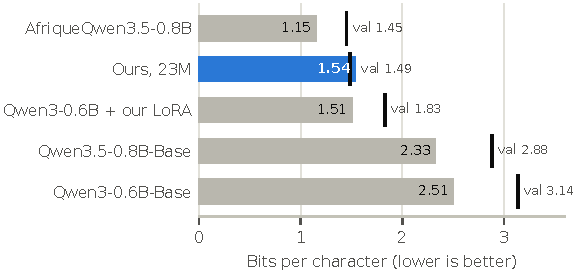
\includegraphics[width=\columnwidth]{figures/open_models.pdf}
\caption{Oromo data matters more than size; Oromo data at larger size is best. Bars: bits per character on 658 held-out Telegram posts from 2026 that no model saw; ticks: validation set.}
\label{fig:open}
\end{figure}

\paragraph{Out-of-the-box Oromo.} The general Qwen3.5 model is far behind our 23M model on every set (2.88 vs.\ 1.49 bits per character on validation; Figure~\ref{fig:open}); prompted with \om{Afaan Oromoo}, it continues in Afrikaans. After African-language continued pretraining, the identical architecture produces fluent Oromo and is the best model on every set. It is close to ours on the validation text (1.45 vs.\ 1.49), which its training data may contain, and clearly ahead on held-out Telegram posts (0.97 vs.\ 1.16) and on the 2026 posts (1.15 vs.\ 1.54). The 2026 posts are the hardest set for our model; a quarter of them are live sports commentary, a style its corpus covers mainly through one channel. Corpus size matters here too: our public-text model scores 1.96 on these posts.

\paragraph{Our own continued pretraining.} We continued pretraining Qwen3-0.6B-Base on 2.5M tokens of our corpus (about 6\% of it) with LoRA: rank-64 adapters on every attention and MLP projection (40M trainable parameters), 49 minutes at about 840 tokens/s. Bits per character fell by 42\% on validation (3.14 to 1.83), 49\% on Telegram (2.63 to 1.36) and 40\% on the 2026 posts (2.51 to 1.51), where the adapted model slightly beats our 23M model (1.51 vs.\ 1.54). It trails ours on the other two sets, and AfriqueQwen, which was adapted with far more data, on all three.

\paragraph{Instruction tuning at 0.8B.} To test whether the shortfall of \S\ref{sec:inst} is one of scale, we instruction-tune AfriqueQwen3.5-0.8B on the same data with the same prompt and prompt masking. LoRA adapters of rank 16 on all attention, linear-attention and MLP projections (10.2M trainable parameters) train for one epoch at learning rate $2\times10^{-4}$, with examples cut to 384 tokens (about 950 characters). Training took about an hour; validation loss on answer tokens is 1.30.

\begin{table}[t]
\centering
\small
\setlength{\tabcolsep}{3.5pt}
\begin{tabular}{@{}llrr@{}}
\toprule
Task & Metric & 23M & 0.8B \\
\midrule
Topic & accuracy & 38.2\% & \textbf{91.1\%} \\
Topic & macro-F1 & 0.41 & \textbf{0.87} \\
Headline & ROUGE-L & 0.063 & \textbf{0.254} \\
Describe & ROUGE-L & 0.084 & \textbf{0.186} \\
\bottomrule
\end{tabular}
\caption{Instruction following on the full test set: our 23M model (\S\ref{sec:inst}) against AfriqueQwen3.5-0.8B with LoRA instruction tuning on the same data. Copying an article's first 10 words as its headline scores ROUGE-L 0.212.}
\label{tab:inst08}
\end{table}

The larger, Oromo-adapted model follows instructions and uses its input (Table~\ref{tab:inst08}). Topic accuracy is 91.1\% and macro-F1 0.87, with F1 of at least 0.73 on every topic (0.80 on technology), and every answer is a valid label. Its headlines beat the copy-the-first-10-words baseline (0.254 vs.\ 0.212). AfriBERTa is public and may be part of AfriqueLLM's pretraining data, so we also score the 244 test headlines that do not appear in it: the margin holds (0.255 vs.\ 0.218). Only 58 of 325 headlines mention Covid-19, against 53 of the real ones. Descriptions of unseen entities improve but remain the weakest task (0.182 without the 14 answers found in AfriBERTa); 3 of 81 degenerate into repetition under greedy decoding. Before instruction tuning, on the first 150 test articles, the same model never produced a valid topic label, although its headline continuations already scored ROUGE-L 0.135. Topic accuracy exceeds our classifier of \S\ref{sec:cls} (87.8\%), but AfriqueLLM's pretraining corpus may contain BBC Afaan Oromoo articles like the MasakhaNEWS test set, which we cannot check, and this result is from a single run.

\paragraph{Compute note.} Training Qwen3.5 on a Mac ran at only 92--290 tokens/s: its linear-attention layers have fast kernels only for NVIDIA GPUs, so PyTorch falls back to a slow reference implementation. We therefore used Qwen3 for our own continued pretraining and kept Qwen3.5 to inference and one epoch of instruction tuning.

\section{Discussion}

For small-scale Oromo modeling, the evidence points to data and tokenization before model size. English-built tokenizers spend about twice as many tokens on Oromo (2.3--2.6 characters per token, against 5.0 for ours), which halves the text a fixed context window can hold. A 23M model trained only on Oromo beats a general 752M model by almost $2\times$ in bits per character, and growing its corpus from 6.9M to 12.8M words improves every held-out set and every downstream task, most of all when few weights are fine-tuned. Size helps once the data is there: with Oromo-rich continued pretraining the 752M model becomes the strongest, and 49 minutes of LoRA on 2.5M tokens bring a general 0.6B model close to ours. Pretraining transfers to topic classification, most strongly for topics with few labeled examples. Instruction following needs more capacity than 23M parameters: better pretraining makes the small model's answers depend more on its input, but it still confuses the tasks, while an Oromo-adapted 0.8B model tuned on the same 3,758 examples follows them. Finally, contamination checks need to look at headlines: the 13-gram test found 1 of 325 test articles in our public-text corpus, while 81 of 325 test headlines were in it.

\section{Conclusion}

A single laptop is enough to build a working Oromo language-modeling pipeline, and the largest gains come from Oromo-specific data and tokenization. A hudhaa-aware 16k tokenizer halves sequence length; a 23M-parameter GPT trained in 77 minutes on 12.8M words outperforms a general 752M model on Oromo and, fine-tuned, beats a strong TF-IDF baseline in macro-F1 on topic classification. Instruction following does not emerge at this scale, but the same instruction data turns an Oromo-adapted 0.8B model into a working Oromo instruction follower on a laptop. Next steps are native-speaker evaluation, more data beyond news, multi-seed instruction tuning of larger Oromo-adapted models, broader benchmarks that include Oromo such as Belebele and SIB-200, and a public release of the tokenizer and of model weights trained on redistributable data.

\section*{Limitations}

The test sets are small (325 news articles, 81 descriptions), so differences of a few points can be noise; we report seed spreads where we can. Generated text and the instruction templates have not been rated by native speakers, and ROUGE-L against one reference is a weak measure of headline quality. The data is mostly news, and Telegram validation posts come from the same channels as the training posts. All training ran on one laptop: pretraining used four passes over the corpus, our continued pretraining saw about 6\% of it, and the faster Qwen3.5 kernels exist only for NVIDIA GPUs. In the corpus-size ablation, data and optimizer steps grow together, and AfriqueQwen and our adapted Qwen3 start from different base models. The 0.8B instruction-tuning result is a single run of one epoch, and AfriqueLLM's pretraining corpus may overlap with the MasakhaNEWS test articles and headlines, which we cannot check. Our filters remove evaluation text from our own training data, but not from public corpora such as AfriBERTa, which other models may have used.

\section*{Ethics Statement}

All public training text comes from public sources. We release code, the trained tokenizer and the cleaning rules (Apache-2.0); AfriBERTa (Apache-2.0), Oromo Wikipedia (CC BY-SA 4.0) and MasakhaNEWS (AFL-3.0) are downloaded by the scripts. Telegram posts remain under their channels' copyright and are not released, nor are weights trained on them; the released importer lets others rebuild the corpus from their own exports, and the public-text model of Table~\ref{tab:lm} can be reproduced without them. The data is mostly news and includes reporting on conflict, politics and public health; some channels belong to political actors or government offices and carry opinion or official messaging rather than independent reporting. Posts can name public figures and private individuals, and we did not test the models for memorization of individual posts. The models are research artifacts for low-resource language modeling and are not suitable for producing news, health information or any content presented as fact.

\section*{Acknowledgments}

This work was carried out with substantial assistance from an AI assistant (Claude, by Anthropic), which wrote much of the code and a first draft of the text under the author's direction. The author directed the project, collected the Telegram data, reviewed the results and takes full responsibility for the content.

\bibliography{references}

\appendix

\section{Reproducibility}
\label{sec:repro}

Every result comes from numbered scripts in the public repository, run on one Apple M1 Max with 64 GB of memory: data preparation (\texttt{01}--\texttt{03}, \texttt{14}, \texttt{21}), tokenizers and encoding (\texttt{04}--\texttt{06}), pretraining (\texttt{07}; 77 minutes, 42--46 for the smaller corpora), its evaluation (\texttt{08}, \texttt{15}), topic classification (\texttt{09}, \texttt{10}; about 30 minutes), instruction tuning (\texttt{11}--\texttt{13}; 15 minutes), open-model comparison (\texttt{16}), LoRA continued pretraining (\texttt{17}; 49 minutes), LoRA instruction tuning and its full-test evaluation (\texttt{18}, \texttt{20}; about 2.5 hours) and the figures (\texttt{19}). Software: PyTorch 2.12 (MPS), Hugging Face \texttt{tokenizers} 0.22, \texttt{transformers} 5.9 and \texttt{peft} 0.21. Pretraining uses seed 123 and classification seeds 1--3; cleaning, splits and sampling are deterministic. The repository's 17 tests cover the tokenizer, data loaders, the model's attention against the book's reference code, the headline filter, and the classification and instruction-tuning data handling. Without Telegram exports, the pipeline reproduces the public-text model.

\end{document}
